
\FullBackgroundPicture{../detector/figures/ring}

\begin{frame}\frametitle{The LHC complex}
\footnotesize\centering
\begin{minipage}{.9\textwidth}
%\end{minipage}\begin{minipage}{.6\textwidth}\centering\pause

\begin{beamercolorbox}[wd=.99\textwidth,rounded=true,shadow=true]{whiteboxcolor}\centering\scriptsize
	\begin{tabular}{lllll}\toprule
        Parameter                       & designed      &       2010 &  2011     &   2012\\ \midrule
\rowcolor{TabLight} Beam energy (\tev/c)            & 7             & 3.5        & 3.5       & 4    \\
        Beta function $\beta*$ (m)      & 0.55          & 2.0/3.5    & 1.5/1.0   & 0.6  \\
        Max. No. bunches/beam           & 2808          & 368        & 1380      &1380  \\
        Max. No. protons/bunch          & 1.15$\times10^{11}$ & 1.2$\times10^{11}$ & 1.45$\times10^{11}$ & 1.7$\times10^{11}$ \\
\rowcolor{TabLight} Bunch spacing (ns)              & 25            & 150       & 75/50        & 50 \\
\rowcolor{TabLight} Peak luminosity (\cmm2\sm1)     & 1$\times10^{34}$& 2.1$\times10^{32}$& 3.7$\times10^{33}$& 7.7$\times10^{33}$\\
        Emittance $\varepsilon_{n}$ ($\mu$rad)&3.75     &   2.0      & 2.4      & 2.5   \\
\rowcolor{TabLight} Max. $<\mu>$                    & 19            & 4             & 17         & 37       \\
	\bottomrule\end{tabular}

\end{beamercolorbox}

\end{minipage}

\myskip

\end{frame}


\FullBackgroundPicture{../detector/figures/atlas}

\begin{frame}\frametitle{The ATLAS Detector}
\footnotesize\centering

\begin{minipage}{.7\textwidth}\centering\pause

\only<2>{
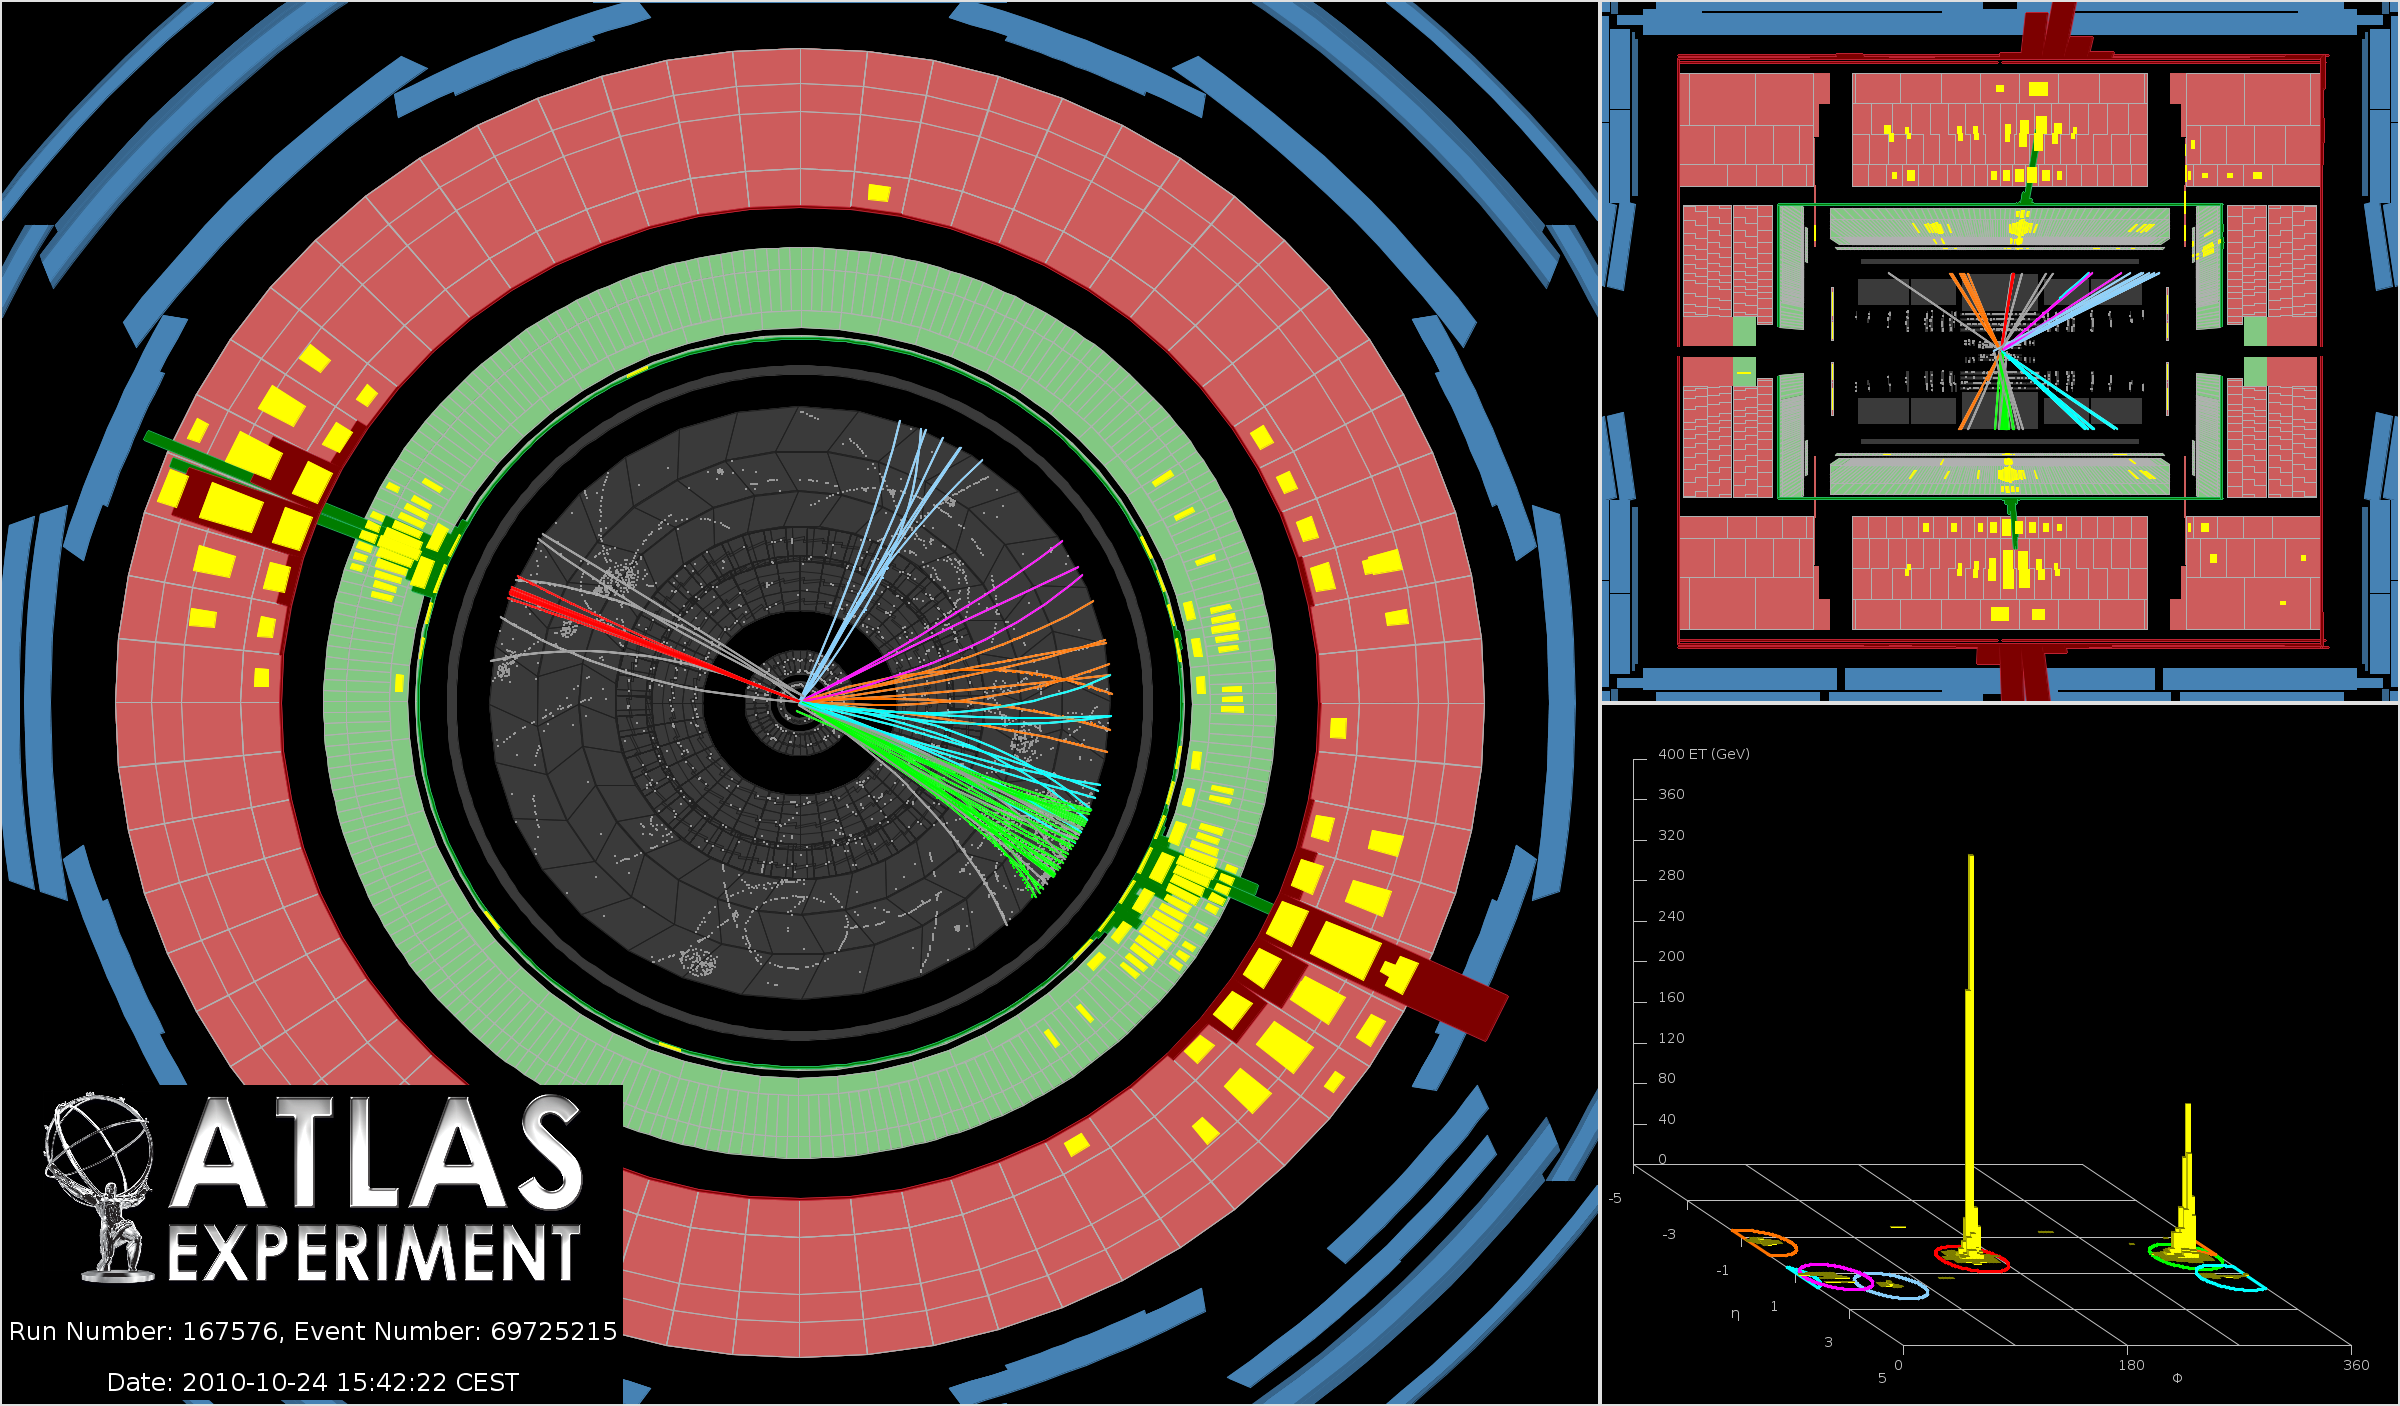
\includegraphics[width=1.\textwidth]{pics/atlasED}
}
\only<3>{
\hspace{2cm}\begin{beamercolorbox}[wd=.9\textwidth,rounded=true,shadow=true]{whiteboxcolor}\centering
{\bfseries In 2012 20.3\ifb\  collected at $\sqrt{s}=8~$TeV!}
\vspace{.3cm}

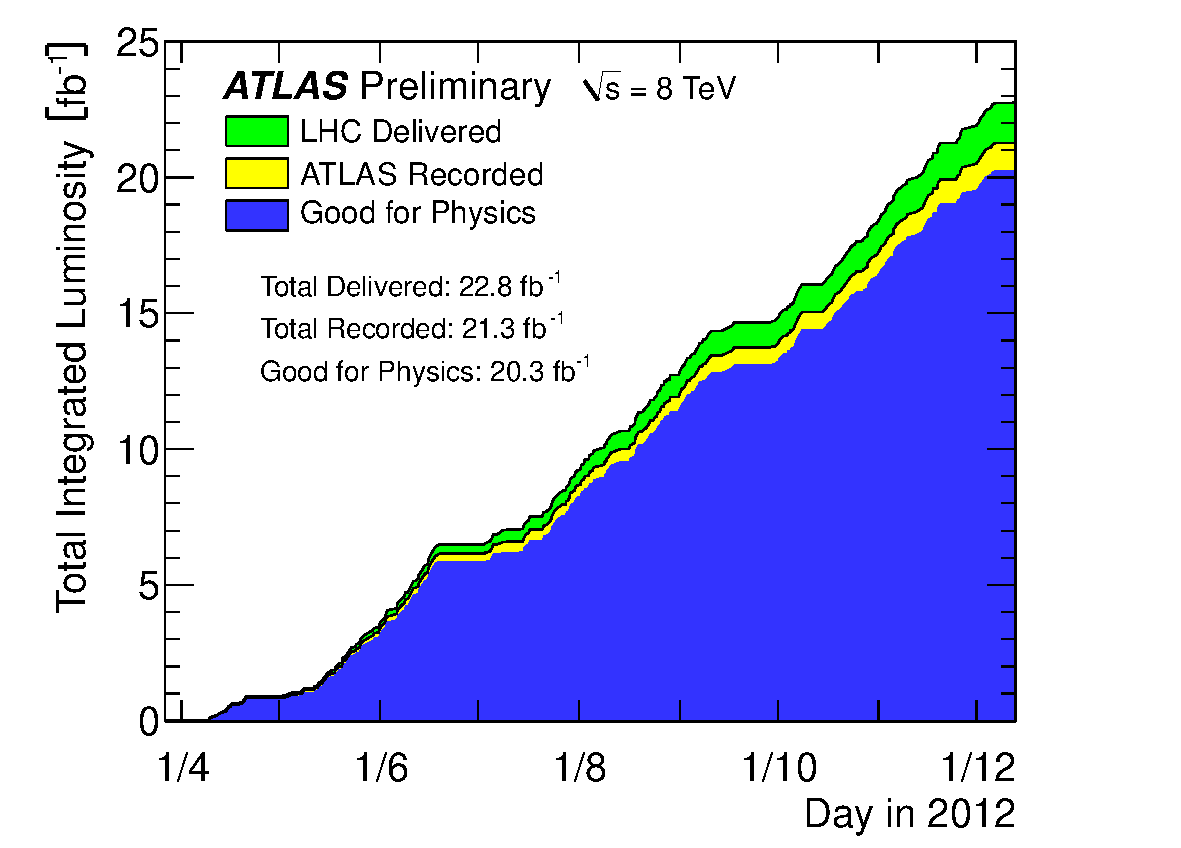
\includegraphics[width=.8\textwidth]{pics/intlumivstime2012DQ}

\vspace{\baselineskip}
%Reached peak luminosity of $3.65\times 10^{33}~$cm$^{-2}$s$^{-1}$\\
\end{beamercolorbox}
}

\end{minipage}

%Will present results obtained with \alert{14.3\ifb}\ of 2012 data

\end{frame}
